%% Creator: Inkscape inkscape 0.48.2, www.inkscape.org
%% PDF/EPS/PS + LaTeX output extension by Johan Engelen, 2010
%% Accompanies image file 'c_comparatore.pdf' (pdf, eps, ps)
%%
%% To include the image in your LaTeX document, write
%%   \input{<filename>.pdf_tex}
%%  instead of
%%   \includegraphics{<filename>.pdf}
%% To scale the image, write
%%   \def\svgwidth{<desired width>}
%%   \input{<filename>.pdf_tex}
%%  instead of
%%   \includegraphics[width=<desired width>]{<filename>.pdf}
%%
%% Images with a different path to the parent latex file can
%% be accessed with the `import' package (which may need to be
%% installed) using
%%   \usepackage{import}
%% in the preamble, and then including the image with
%%   \import{<path to file>}{<filename>.pdf_tex}
%% Alternatively, one can specify
%%   \graphicspath{{<path to file>/}}
%% 
%% For more information, please see info/svg-inkscape on CTAN:
%%   http://tug.ctan.org/tex-archive/info/svg-inkscape
%%
\begingroup%
  \makeatletter%
  \providecommand\color[2][]{%
    \errmessage{(Inkscape) Color is used for the text in Inkscape, but the package 'color.sty' is not loaded}%
    \renewcommand\color[2][]{}%
  }%
  \providecommand\transparent[1]{%
    \errmessage{(Inkscape) Transparency is used (non-zero) for the text in Inkscape, but the package 'transparent.sty' is not loaded}%
    \renewcommand\transparent[1]{}%
  }%
  \providecommand\rotatebox[2]{#2}%
  \ifx\svgwidth\undefined%
    \setlength{\unitlength}{167.7234375bp}%
    \ifx\svgscale\undefined%
      \relax%
    \else%
      \setlength{\unitlength}{\unitlength * \real{\svgscale}}%
    \fi%
  \else%
    \setlength{\unitlength}{\svgwidth}%
  \fi%
  \global\let\svgwidth\undefined%
  \global\let\svgscale\undefined%
  \makeatother%
  \begin{picture}(1,0.8680247)%
    \put(0,0){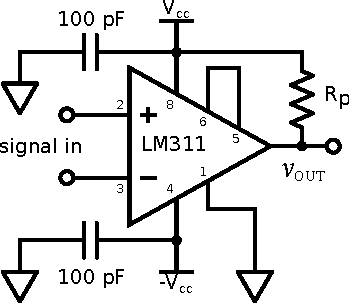
\includegraphics[width=\unitlength]{c_comparatore.pdf}}%
    \put(0.46065586,0.82629864){\makebox(0,0)[lb]{\smash{V}}}%
    \put(0.49978278,0.81485122){\makebox(0,0)[lb]{\smash{cc}}}%
    \put(0.45111636,0.03928878){\makebox(0,0)[lb]{\smash{-V}}}%
    \put(0.50757091,0.02784136){\makebox(0,0)[lb]{\smash{cc}}}%
    \put(-0.00678028,0.43040884){\makebox(0,0)[lb]{\smash{signal in}}}%
    \put(0.32710266,0.5544225){\makebox(0,0)[lb]{\smash{2384561}}}%
    \put(0.16016122,0.05359807){\makebox(0,0)[lb]{\smash{100 pF
100 pF}}}%
    \put(0.80407833,0.36363224){\makebox(0,0)[lb]{\smash{v}}}%
    \put(0.83895729,0.34836903){\makebox(0,0)[lb]{\smash{OUT}}}%
    \put(0.92332219,0.57827127){\makebox(0,0)[lb]{\smash{RpLM311}}}%
    \put(0.80131908,0.82039821){\makebox(0,0)[lb]{\smash{+5V}}}%
  \end{picture}%
\endgroup%
